\RequirePackage{luatex85}
\pdfminorversion=7
\documentclass[screen]{../../../../sty/open-logic-book}
\usepackage[all]{nowidow}
\usepackage[no-math]{fontspec}
\newcommand{\olpath}{../../../..}
\defaultfontfeatures{Renderer=HarfBuzz,Script=Gujarati}
\setmainfont{NotoSansGujarati-Regular.ttf}[
  Path=\olpath/fonts/,BoldFont=NotoSansGujarati-Bold.ttf,
  ItalicFont=NotoSansGujarati-Regular.ttf,ItalicFeatures={FakeSlant=.15},
  BoldItalicFont=NotoSansGujarati-Bold.ttf,BoldItalicFeatures={FakeSlant=.15}]
\setsansfont{NotoSansGujarati-Regular.ttf}[
  Path=\olpath/fonts/,BoldFont=NotoSansGujarati-Bold.ttf,
  ItalicFont=NotoSansGujarati-Regular.ttf,ItalicFeatures={FakeSlant=.15},
  BoldItalicFont=NotoSansGujarati-Bold.ttf,BoldItalicFeatures={FakeSlant=.15}]
\setmonofont{NotoSansGujarati-Regular.ttf}[
  Path=\olpath/fonts/,BoldFont=NotoSansGujarati-Bold.ttf]
\definecolor{OLPcolor}{RGB}{248,154,14}
\definecolor{OLPdkcolor}{RGB}{104,65,6}
\definecolor{OLPltcolor}{RGB}{248,203,137}

\usepackage[nonumberlist,toc,style=index,nopostdot]{glossaries}
\makeglossaries
\NewDocumentCommand\slcterm{O{} m m m m}{%
  \newglossaryentry{#2}{sort={#3},name={#4},plural={#4},
    symbol={#1},description={#5}}}

\def\oljobname{slc}
\newcommand*{\ollangid}{gu}
\newcommand*{\ollanguage}{gujarati}
\PassOptionsToPackage{provide=*}{babel}
\input{\olpath/sty/open-logic.sty}
\renewcommand{\gitissue}[1]{\href{https://github.com/OpenLogicProject/OpenLogic/issues/#1}{મુદ્દો \##1}}
\RenewDocumentCommand{\olasset}{O{\olphotowidth} m}{%
  \begin{center}\resizebox{#1}{!}{%
    \IfFileExists{#2}{\input{#2}}{\input{\olpath/#2}}}%
  \end{center}}
\tikzset{initial text=પ્રારંભ}
\setOLPbooktitle[ગણો,\protect\\ તર્ક,\protect\\ સંગણન]{ગણો, તર્ક, સંગણન}
\setOLPbooksubtitle{અધિતર્કનો મુક્ત પરિચય}
\setOLPauthor{Richard Zach}
\setOLPbookversion{ગુજરાતી આવૃત્તિ}{gu-Gujr-IN}
\setOLPsourcelink{https://slc.openlogicproject.org/}
\setOLPauthorlink{https://richardzach.org/}
\renewcommand*{\OLPtitlecoverfont}{\fontsize{44pt}{53pt}\sffamily\bfseries}
\renewcommand*{\OLPsubtitlecoverfont}{\fontsize{20pt}{25pt}\sffamily\bfseries}
\renewcommand*{\olremixedby}{%
  રચના અને સંપાદન \OLPauthor{}\\
  Open Logic Projectના કાર્ય પર આધારિત\\[.4em]
  પુસ્તક-વિશિષ્ટ ગુજરાતી અનુવાદ કૃત્રિમ બુદ્ધિથી તૈયાર થયો છે.\\
  OpenAI Codex, GPT-6.1 Sol (Ultra)\\
  સમાવેલો પાઠ ગુજરાતી Open Logic આવૃત્તિમાંથી છે.\\
  પાઠ CC BY 4.0 પરવાના હેઠળ છે.}

\renewcommand*{\olacknowledgements}{%
  Open Logic Project કૅલ્ગરી યુનિવર્સિટીની
  \href{https://taylorinstitute.ucalgary.ca/}{Taylor Institute of Teaching and Learning}
  અને આલ્બર્ટા સરકારના સમર્થનથી ચાલતા Alberta Open Educational Resources
  (ABOER) Initiativeનો આભાર માને છે.}

\renewcommand*{\olillustrations}{%
  મુખપૃષ્ઠનાં અને ભાગોના આરંભનાં ચિત્રો
  \href{https://github.com/OpenLogicProject/portraits}{Matthew Leadbeater}નાં છે.
  તે \href{https://creativecommons.org/licenses/by-nc/4.0/}{CC BY-NC 4.0}
  હેઠળ વપરાયાં છે. ફોટોગ્રાફનો શ્રેય અને વપરાશની શરતો સંબંધિત વિભાગમાં છે.}

\renewcommand*{\olcolophon}{%
  Noto Sans Gujarati અક્ષરરૂપમાં Lua\LaTeX{}થી અક્ષરાંકન.}

\renewcommand*{\olbookrevision}{%
  Richard Zachના પુસ્તકનો સ્રોત
  \href{https://github.com/rzach/sets-logic-computation/tree/6178f32f61645f3b62ef621b4c5a88f8e67778ad}{6178f32}
  આવૃત્તિ છે. Open Logic Projectનો સ્રોત
  \href{https://github.com/OpenLogicProject/OpenLogic/tree/9620cc73f9c8e0ad003c514a5d3748f29611c4c0}{9620cc73}
  આવૃત્તિ છે. મૂળ પુસ્તક \url{\OLPsourcelink} પરથી મફત ઉતારી શકાય છે.}

\renewcommand*{\ollicensetext}[3]{%
  #2નું \textit{#1} પુસ્તક #3 પરવાના હેઠળ છે.}
\renewcommand*{\oluselicensetext}{%
  આ પુસ્તક \href{https://openlogicproject.org/}{\OLPname}ના
  \textit{\href{\OLTlinkname}{\OLTname}} પર આધારિત છે. મૂળ પાઠ
  \href{https://creativecommons.org/licenses/by/4.0/}{\licensename}
  હેઠળ વપરાયો છે.}

% Back-cover copy shared by the 6 × 9 and Lulu Royal upstream formats.
\newcommand*{\slcbackcover}{%
  Richard Zachનું \textit{ગણો, તર્ક, સંગણન}
  \href{https://creativecommons.org/licenses/by/4.0/}{CC BY 4.0}
  આંતરરાષ્ટ્રીય પરવાના હેઠળ છે. આ પુસ્તક Open Logic Projectના
  \textit{ધ ઓપન લોજિક ટેક્સ્ટ} (\url{https://openlogicproject.org/})
  પર આધારિત છે. એ પાઠ પણ CC BY 4.0 હેઠળ વપરાયો છે.}
\newcommand*{\slcprintcredit}{સંપાદક Richard Zach}

\renewcommand*{\oluselicense}[2]{%
  \begin{minipage}[b]{.9cm}
    \includegraphics[width=.9cm]{\olpath/assets/logos/by}
    \includegraphics[width=.9cm]{\olpath/assets/logos/cc}
    \includegraphics[width=.9cm]{\olpath/assets/logos/remix}
  \end{minipage}\hspace{.3cm}%
  \begin{minipage}[b]{5cm}
    \ollicensefont\slcbackcover
  \end{minipage}\hfill
  \href{https://openlogicproject.org/}{\includegraphics[width=2.7cm]{\olpath/assets/logos/openlogic-logo-bw}}}


\input{\olpath/sty/open-logic-defer.sty}
\loadglsentries{include/glossary}
\hypersetup{unicode=true}
\usepackage{truncate}
\AtBeginDocument{%
  \makeoddhead{OLPpage}{\slcchaptermark}{}{\slcpagefolio}%
  \makeevenhead{OLPpage}{\slcchaptermark}{}{\slcpagefolio}}
\newcommand*{\slcchaptermark}{%
  \small\sffamily\color{OLPdkcolor}\truncate{.85\textwidth}{\leftmark}}
\newcommand*{\slcpagefolio}{\sffamily\bfseries\color{OLPdkcolor}\thepage}
\emergencystretch=2em
\errorcontextlines=20

\begin{document}
\raggedbottom
\OLPscreencover{%
  \hfill\hspace{.29\textwidth}\includegraphics[width=.26\textwidth]{\olpath/assets/portraits/cantor-circle.pdf}\hfill{}

  \hfill{}
  \includegraphics[width=.26\textwidth]{\olpath/assets/portraits/goedel-circle.pdf}
  \hfil\includegraphics[width=.26\textwidth]{\olpath/assets/portraits/turing-circle.pdf}\hfil{}
  \includegraphics[width=.26\textwidth]{\olpath/assets/portraits/skolem-circle.pdf}
  \hfill{}

  \hfill{}
  \includegraphics[width=.26\textwidth]{\olpath/assets/portraits/noether-circle.pdf}\hspace{.29\textwidth}\hfill{}
}
\preto\OLEndChapterHook{%
  \IfFileExists{include/summary-\thechapter.tex}{%
    \section*{સારાંશ}\addcontentsline{toc}{section}{સારાંશ}%
    \let\emph\textbf\input{include/summary-\thechapter}\let\emph\textit}{}}
\problemsperchapter

\frontmatter
\OLPfrontmatter

\cleartoverso
\thispagestyle{empty}
\ \vfill
\noindent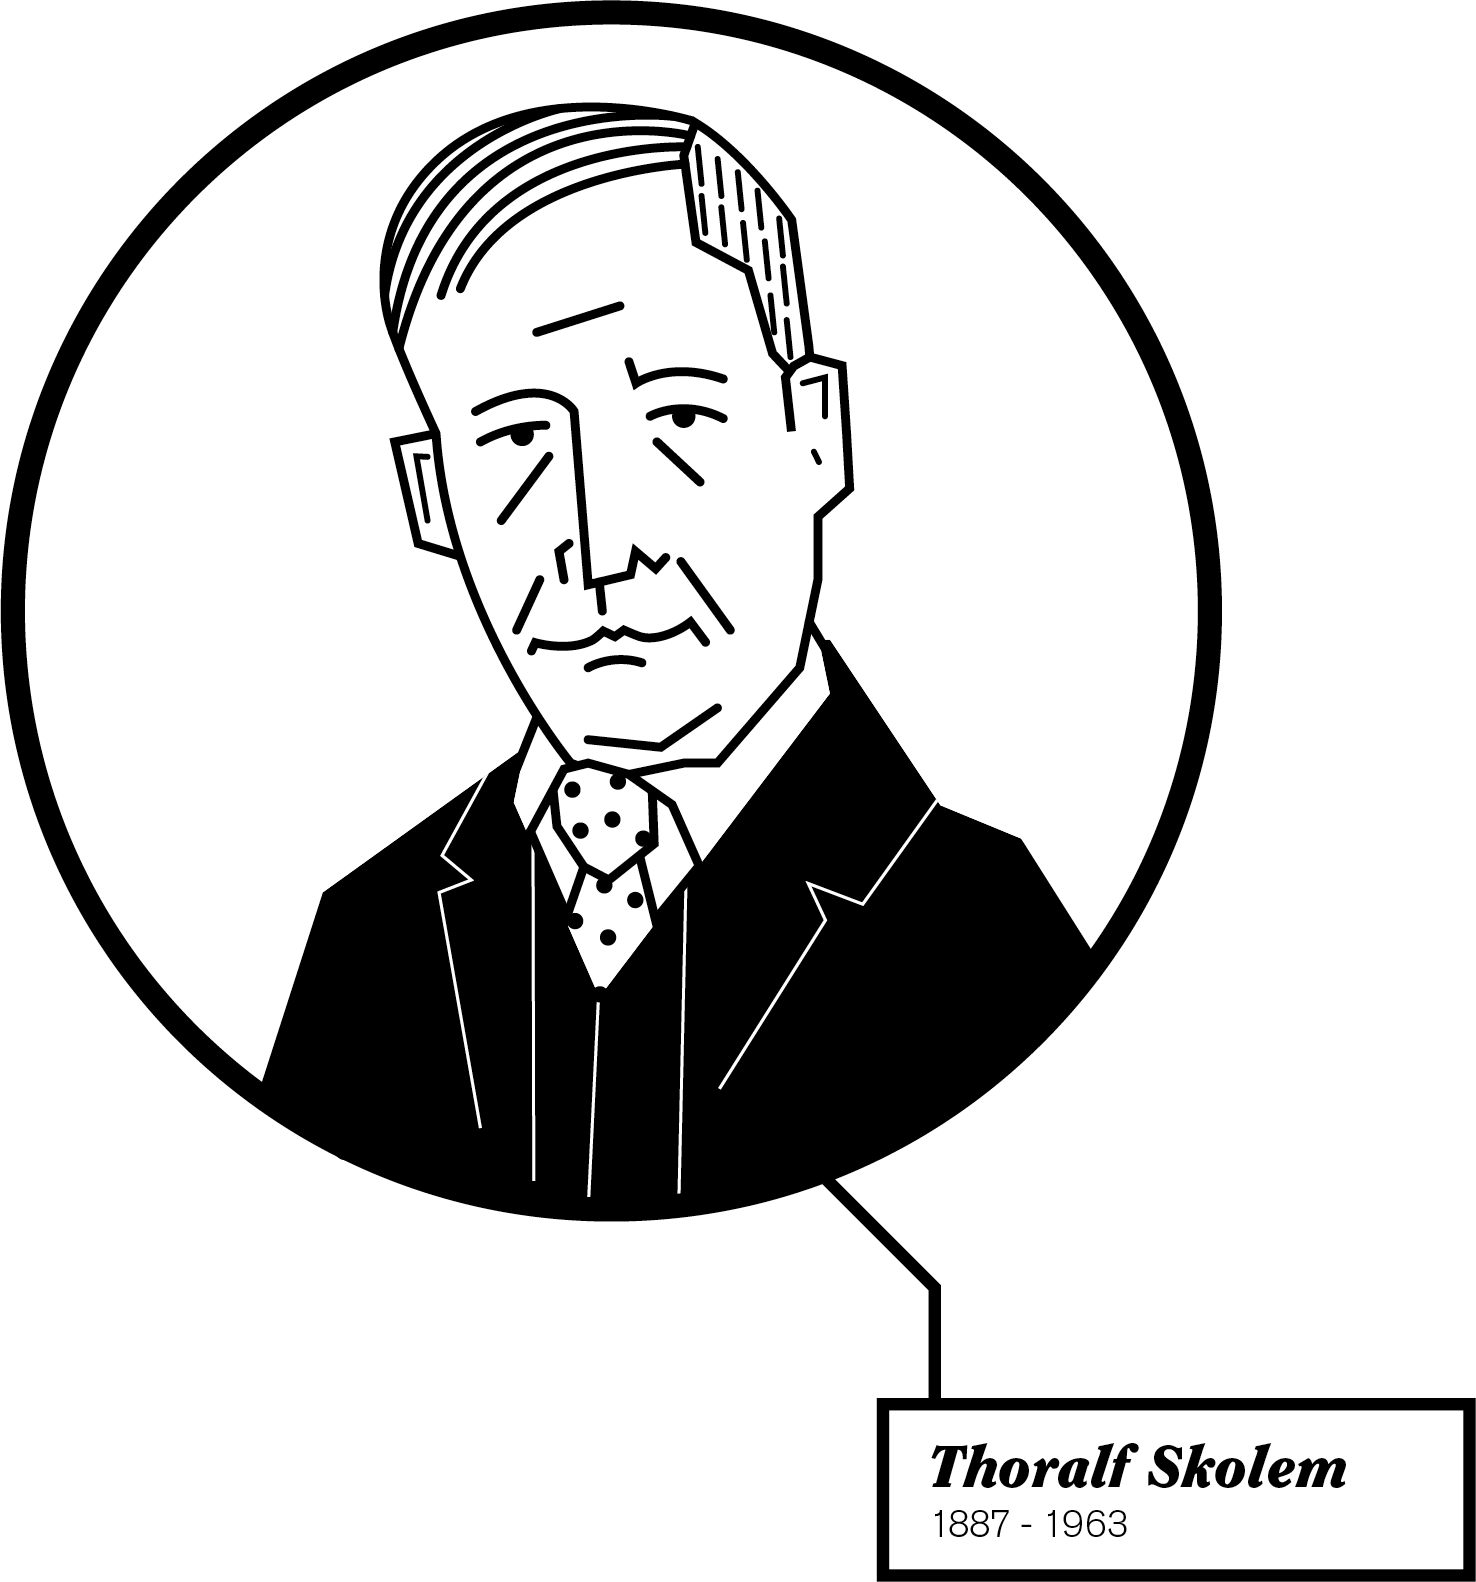
\includegraphics[width=\textwidth]{illustrations/SkolemChapter}
\vfill
\chapter{પ્રસ્તાવના}

આ પુસ્તક અધિતર્કનો પરિચય આપે છે. તે ખાસ કરીને સંગણકવિજ્ઞાન અને
તત્ત્વજ્ઞાનના વિદ્યાર્થીઓ માટે લખાયું છે. «અધિતર્ક» નામ એટલા માટે છે
કે એ વિદ્યાશાખા તર્કનો પોતાનો જ અભ્યાસ કરે છે. તર્કનો વિષય માન્ય
અનુમાનના નિયમો છે. તેનું સાંકેતિક અથવા ઔપચારિક સ્વરૂપ આ નિયમોને
વિધાનતર્ક અને પ્રથમ-ક્રમ તર્ક જેવી ઔપચારિક ભાષાઓમાં રજૂ કરે છે. અધિતર્ક
આ ભાષાઓના અને એમનો ઉપયોગ કરતા સાચા અનુમાનના નિયમોના ગુણધર્મો તપાસે છે.
એવી ભાષાઓના અભિવ્યંજકોને ચોક્કસ અર્થ કેવી રીતે આપવો, માન્ય અનુમાનના
નિયમોનો આધાર કેવી રીતે આપવો અને વિવિધ નિષ્પત્તિ-પ્રણાલીઓના સંગણકીય
તેમજ અન્ય ગુણધર્મો કયા છે, એવા વિષયો તેમાં આવે છે. આ પ્રશ્નો પોતે જ
અગત્યના અને રસપ્રદ છે. આપણે જે ભાષાઓ અને નિષ્પત્તિ-પ્રણાલીઓ તપાસીએ
છીએ તે ખાસ કરીને ગણિત, તત્ત્વજ્ઞાન, સંગણકવિજ્ઞાન અને ભાષાવિજ્ઞાનમાં
વપરાય છે. ઔપચારિક પ્રણાલીઓનો સામાન્ય રીતે અભ્યાસ કેવી રીતે કરવો તેનાં
ઉદાહરણો પણ એમાંથી મળે છે. અહીં આપણે જે તાર્કિક ભાષાઓ ભણીએ છીએ એ ઉપરાંત
બીજી ભાષાઓ પણ રસના વિષય છે. દાખલા તરીકે, ભાષાવિજ્ઞાનીઓ અને
તત્ત્વજ્ઞાનીઓને વિધાનતર્ક તથા પ્રથમ-ક્રમ તર્કની ભાષાઓ કરતાં ઘણી જટિલ
ભાષાઓમાં રસ છે. સંગણકવિજ્ઞાનીઓને કાર્યક્રમલેખનની ભાષાઓ જેવા સાવ જુદા
\emph{પ્રકારો}માં રસ છે. અહીં ચર્ચેલી પદ્ધતિઓ ત્યાં પણ લાગુ પડે છે.
ઔપચારિક ભાષાનું અર્થવિજ્ઞાન કેવી રીતે આપવું, તેના વિશેનાં પરિણામો કેવી
રીતે સાબિત કરવાં અને તેના ગુણધર્મો કેવી રીતે તપાસવા, તે આ પદ્ધતિઓ
બતાવે છે.

બીજી વિદ્યાશાખાઓની જેમ અધિતર્ક પાસે પણ પરિણામો અને તથ્યો છે, અને
પદ્ધતિઓ તથા પ્રયુક્તિઓનો ભંડાર છે. આ પાઠ્યપુસ્તકમાં બંનેનો સમાવેશ છે.
ઘણા વિદ્યાર્થીઓને અભ્યાસક્રમની બહાર અહીં ચર્ચેલાં બધાં પરિણામો જાણવાની
જરૂર નહીં પડે, પણ એ સ્થાપિત કરવાની પદ્ધતિઓની જરૂર પડશે અને તેઓ તેનો
ઉપયોગ કરશે. દાખલા તરીકે, સંગણકવિજ્ઞાનમાં લેવેનહાઇમ--સ્કોલેમ પ્રમેય
વારંવાર આવતું નથી, પણ તેને સાબિત કરવા વાપરેલી પદ્ધતિઓ ત્યાં વપરાય છે.
આમાંનાં ઘણાં પરિણામો વિજ્ઞાનના તત્ત્વજ્ઞાન અને તત્ત્વમીમાંસા જેવી
શાખાઓના અમુક વિવાદોમાં પણ પ્રસ્તુત છે. તત્ત્વજ્ઞાનના વિદ્યાર્થીઓએ આ
અભ્યાસક્રમની બહાર એ પરિણામો સાબિત કરવાં પડે એવું જરૂરી નથી, પણ
પરિણામો શું કહે છે તે સમજવું પડશે. તેમને સ્થાપિત કરવા માટેની વ્યાખ્યાઓ
અને સાબિતીઓ પર વિચાર કર્યો હોય ત્યારે જ એ પરિણામો ખરેખર \emph{સમજાય}
છે. સંગણકવિજ્ઞાન અને તત્ત્વજ્ઞાનના વિદ્યાર્થીઓને આ પુસ્તકનાં પરિણામો અને
પદ્ધતિઓનો અભ્યાસ કરવાની ભલામણ કરવામાં આવે છે, અને અમુક સંજોગોમાં તે
ફરજિયાત પણ હોય છે. આ તેનાં કેટલાંક કારણો છે.

સામગ્રી ત્રણ ભાગમાં વહેંચાઈ છે. \Olref[sfr][][]{part}માં ગણસિદ્ધાંતની
ચર્ચા છે. ઐતિહાસિક રીતે તર્ક અને અધિતર્કનો «ગણિતના પાયા» સાથે ઘણો
ગાઢ સંબંધ છે. પૂર્ણાંકો, પરિમેય અને વાસ્તવિક સંખ્યાઓ, ફલનો, અવકાશો
જેવી ગણિતીય વસ્તુઓને છેવટે કેવી રીતે સમજવી એ ગણિતના પાયાનો પ્રશ્ન
છે. ગણસિદ્ધાંત તેનો એક ઉત્તર આપે છે. બીજા ઉત્તરો પણ છે. તેથી
ગણસિદ્ધાંત અને તર્કનો અભ્યાસ લાંબા સમયથી સાથે થયો છે. ગણ, સંબંધ અને
ફલન ગણિતમાં, સંગણકવિજ્ઞાનમાં તથા તત્ત્વજ્ઞાનના વધુ તકનીકી ક્ષેત્રોમાં
અનેક પ્રકારની ઔપચારિક તપાસમાં સર્વત્ર જોવા મળે છે. તર્કના અર્થવિજ્ઞાન,
સાબિતી-સિદ્ધાંત અને સંગણનીયતાના પાયાનાં પરિણામો ઘડવા અને સાબિત કરવા
માટે ચોક્કસ પરિભાષા અનિવાર્ય છે. દાખલા તરીકે, આપણે અભિવ્યંજકોના ગણો,
તાર્કિક પરિણામ અને સાબિતીક્ષમતાના સંબંધો, વિધેયચિહ્નોના અર્થઘટનો
(જે સંબંધો હોય છે), સંગણનીય ફલનો અને તેમની વચ્ચેના સંબંધો તથા એમના
પરથી થતી રચનાઓની વાત કરીશું. તે માટે ટૂંકાં સંકેતો રાખવા અને ગણો,
સંબંધો તથા ફલનોના સામાન્ય ગુણધર્મો પર વિચાર કરવો ઉપયોગી છે. ગણિતીય
વિચાર અને સાબિતીઓ ઘડવાનો અનુભવ ઓછો હોય તો ગણસિદ્ધાંતનો પહેલો ભાગ
અભ્યાસ માટેનું મેદાન સમજો. બધી મૂળભૂત વ્યાખ્યાઓ આપવામાં આવશે અને
તેમની મદદથી ક્રમે વધુ જટિલ સાબિતીઓ આપીશું. ખાસ કરીને પહેલા ભાગમાં
પરિણામો સમજવા કરતાં કદાચ સાબિતીઓ સમજવી અને જાતે શોધીને ઘડતાં શીખવું
વધુ અગત્યનું છે. ગણિતીય વિચારસરણી નવી હોય તો ઉદાહરણો અને સ્વાધ્યાયો
જાતે વિચારીને કરવા અગત્યનું છે.

પહેલા ભાગમાં એક અગત્યનું પરિણામ પણ સ્થાપિત કરીશું, કૅન્ટૉરનું પ્રમેય.
તે વિજ્ઞાનોમાં ખ્યાલ-વિશ્લેષણનાં સૌથી નોંધપાત્ર ઉદાહરણોમાંના એક પર
આધારિત છે, એટલે કે કૅન્ટૉરે કરેલું અનંતતાનું વિશ્લેષણ. સદીઓથી અનંતતાએ
ગણિતજ્ઞો અને તત્ત્વજ્ઞાનીઓ બંનેને મૂંઝવ્યા છે. કૅન્ટૉર પહેલાં તેના વિશે
યોગ્ય રીતે વિચારવાની રીત કોઈ જાણતું નહોતું. ઘણા તો તેના વિશે વિચારવું
જ ભૂલ માનતા અને અનંત સંગ્રહનો ખ્યાલ જ અસંગત હોવાનું માનતા. કૅન્ટૉરે
અનંતતાને સુસંગત રીતે અભ્યાસ કરી શકાય એવો વિષય બનાવ્યો. તેમણે અનંત
સંગ્રહોનો અને તેમનાં કદ માપવા માટેની અનંત સંખ્યાઓનો આખો સિદ્ધાંત
વિકસાવ્યો. તેમણે બતાવ્યું કે અનંતતાનાં જુદાં સ્તરો હોય છે. «પરિમિતાતીત»
સંખ્યાઓનો આ સિદ્ધાંત સુંદર અને અટપટો છે. આપણે તેમાં બહુ ઊંડે નહીં
ઊતરીએ, પણ બતાવી શકીશું કે અનંતતાનાં જુદાં સ્તરો હોય છે, ખાસ કરીને
«ગણનીય» અને «અગણનીય» અનંતતા. આ પરિણામના અગત્યના ઉપયોગો છે અને તે
દરેક ગણિતજ્ઞ, સંગણકવિજ્ઞાની અને તત્ત્વજ્ઞાને જાણવા જેવું પરિણામ પણ છે.

\olref[fol][][]{part}માં આપણે પ્રથમ-ક્રમ તર્ક તરફ વળીએ છીએ. પ્રથમ-ક્રમ
તર્કની ભાષા અને તેનું અર્થવિજ્ઞાન વ્યાખ્યાયિત કરીશું, એટલે કે પ્રથમ-ક્રમની
સંરચનાઓ શું છે અને એ તર્કનું વાક્ય સંરચનામાં ક્યારે સાચું છે. તેનાથી બે
અગત્યનાં કામ થઈ શકશે. (1) એક વાક્ય બીજા વાક્યનું તાર્કિક પરિણામ
ક્યારે છે તેની ગણિતીય રીતે ચોક્કસ વ્યાખ્યા આપી શકીશું. (2) પ્રથમ-ક્રમની
સંરચના બનાવતા સંબંધોને એ સંરચનામાં સાચાં હોય તે વાક્યો કેવી રીતે
લક્ષણબદ્ધ કરે છે તે જોઈ શકીશું. તે ખાસ કરીને સ્વયંસિદ્ધીય પદ્ધતિની
ચર્ચા તરફ દોરી જાય છે. એ પદ્ધતિમાં અમુક પ્રકારની સંરચનાઓનું લક્ષણ
આપવા પ્રથમ-ક્રમની ભાષાનાં વાક્યો વપરાય છે. પછી સાબિતી-સિદ્ધાંત
લઈશું અને ગેરહાર્ડ ગેન્ટ્સેને 1930ના દાયકામાં આપેલાં સિક્વન્ટ કલન
અને સ્વાભાવિક નિગમનનાં મૂળ સ્વરૂપો જોઈશું. (તમારા અધ્યાપક ફક્ત એક પ્રણાલી
પસંદ કરે તો «નિષ્પત્તિ» અને «નિષ્પન્નક્ષમતા»નો ઉલ્લેખ તે પ્રણાલી
માટે સમજવો.) તાર્કિક પરિણામનો અર્થવિષયક ખ્યાલ અને નિષ્પન્નક્ષમતાનો
વાક્યરચનાત્મક ખ્યાલ, કોઈ વાક્ય બીજાં વાક્યોમાંથી ફલિત થાય છે એ વાતને
ચોક્કસ બનાવવાની સાવ જુદી બે રીતો છે. યથાર્થતા અને પૂર્ણતાનાં પ્રમેયો
આ બંને લક્ષણોને સાંકળે છે. ખાસ કરીને, આપણે ગેડલનું પૂર્ણતા પ્રમેય
સાબિત કરીશું. તે કહે છે કે જો કોઈ વાક્ય બીજાં વાક્યોનું અર્થવિષયક
તાર્કિક પરિણામ હોય તો તે એમનામાંથી નિષ્પન્ન પણ કરી શકાય છે. તેનું
એક સમકક્ષ સ્વરૂપ એ છે કે જો વાક્યોનો સંગ્રહ સુસંગત હોય, એટલે કે
તેનામાંથી કોઈ વિરોધાભાસ સાબિત કરી શકાતો ન હોય, તો એવી સંરચના છે
જેમાં એ બધાં વાક્યો સાચાં હોય.

પૂર્ણતા પ્રમેયનું બીજું સ્વરૂપ કદાચ વધુ આશ્ચર્યજનક છે. ગેડલે આ પરિણામ
સાબિત કર્યું એ અરસામાં (1929માં) જર્મન ગણિતજ્ઞ ડાવિડ હિલ્બર્ટનો જાણીતો
મત હતો કે ગણિતીય અસ્તિત્વ માટે સુસંગતતા, એટલે કે વિરોધાભાસનો અભાવ,
પૂરતી છે. બીજા શબ્દોમાં, જ્યારે ગણિતજ્ઞ સંરચના કે સંરચનાઓના વર્ગનું
સુસંગત વર્ણન કરી શકે ત્યારે તેમને એવી સંરચનાઓના અસ્તિત્વમાં વિશ્વાસ
રાખવાનો અધિકાર છે. એ વખતે ઘણાને આ વિચાર વાહિયાત લાગતો. પોતાની
વાતમાં વિરોધાભાસ કર્યા વિના સંરચનાનું વર્ણન કરી શકાય એટલાથી એવી
સંરચના ખરેખર અસ્તિત્વ ધરાવે છે એમ શી રીતે નીકળે? ગેડલનું પૂર્ણતા
પ્રમેય બરાબર આ જ કહે છે. આ વિરોધાભાસ જેવું જણાતું અને તત્ત્વજ્ઞાનની
દૃષ્ટિએ રસપ્રદ પાસું ઉપરાંત, પૂર્ણતા પ્રમેયના બે અગત્યના ઉપયોગ છે.
તેનાથી આપેલાં વાક્યોને સાચાં કરતી સંરચનાઓના અસ્તિત્વ વિશે વધુ પરિણામો
સાબિત કરી શકાય છે. આ પરિણામો સઘનતા પ્રમેય અને
લેવેનહાઇમ--સ્કોલેમ પ્રમેય છે.

\olref[tur][][]{part}માં આપણે તર્કને સંગણનીયતા સાથે સાંકળીએ છીએ. અહીં
પણ ઐતિહાસિક સંબંધ છે. તર્કનું આપેલું વાક્ય સાબિતી ધરાવે છે કે કેમ
તે નક્કી કરતી યાંત્રિક પદ્ધતિ શોધવાનો પ્રશ્ન ડાવિડ હિલ્બર્ટે તર્કના
મૂળ પ્રશ્ન તરીકે મૂક્યો હતો. વિધાનતર્કમાં આવી પદ્ધતિ છે. બધી સત્યતા
સારણીઓ તપાસવાની છે અને તે સાન્ત સંખ્યામાં હોવાથી અંતે સાચો ઉત્તર
મળે છે. પ્રથમ-ક્રમ તર્ક માટે આવી સીધી પદ્ધતિ શક્ય નથી. શક્ય
સંરચનાઓની સંખ્યા અનંત છે, અને સંરચનાઓ પોતે પણ અનંત હોઈ શકે છે.
તર્કશાસ્ત્રીઓ વર્ષો સુધી વધુ કુશળ પદ્ધતિ શોધતા રહ્યા. છેવટે અલૉન્ઝો
ચર્ચ અને એલન ટ્યુરિંગે સ્થાપિત કર્યું કે એવી કોઈ પદ્ધતિ નથી. એ કરવા
માટે પહેલાં યાંત્રિક પદ્ધતિની સામાન્ય અને ચોક્કસ વ્યાખ્યા આપવી જરૂરી
હતી. કોઈ નિર્ણયવિધિ સૂચવાઈ હોત તો કદાચ લોકો તેને અસરકારક પદ્ધતિ
તરીકે ઓળખી શક્યા હોત. કોઈ અસરકારક પદ્ધતિ અસ્તિત્વમાં નથી એવું
સાબિત કરવા પહેલાં «અસરકારક પદ્ધતિ» વ્યાખ્યાયિત કરવી પડે અને એ
વ્યાખ્યાના આધારે અશક્યતાની સાબિતી આપવી પડે. ટ્યુરિંગે એમ જ કર્યું.
સૈદ્ધાંતિક રીતે યાંત્રિક પ્રક્રિયા શું કરી શકે તેનો ગણિતીય નિદર્શ
તરીકે તેમણે ટ્યુરિંગ મશીનનો વિચાર આપ્યો.\footnote{ટ્યુરિંગે પોતે
અલબત્ત તેને એ નામ આપ્યું નહોતું.} ગણિતીય સાધનો વડે અનૌપચારિક ખ્યાલનું
\emph{ખ્યાલ-વિશ્લેષણ} કરવાનું આ બીજું ઉદાહરણ છે. સંગણકવિજ્ઞાન માટે
તેનું મહત્ત્વ કદાચ ગણિત માટે કૅન્ટૉરના અનંતતાના વિશ્લેષણ જેટલું છે.
આપણું છેલ્લું મુખ્ય કાર્ય બે અશક્યતા પ્રમેયોની સાબિતીનું રહેશે.
ટ્યુરિંગ મશીનો વડે કહેવાતી «અટકવાની સમસ્યા» ઉકેલી શકાતી નથી અને
અંતે હિલ્બર્ટની તર્ક માટેની «નિર્ણય સમસ્યા» પણ ઉકેલી શકાતી નથી, એ
બતાવીશું.

આ પાઠ ગણિતીય છે, કારણ કે આપણે ગણિતીય વ્યાખ્યાઓની ચર્ચા કરીએ છીએ અને
પરિણામો ગણિતીય રીતે સાબિત કરીએ છીએ. તે માટે ગણિતની વિસ્તૃત પૂર્વજાણકારીની
જરૂર નથી. પાઠમાં કશા માટે બીજગણિત, ત્રિકોણમિતિ કે કલન જાણવાની જરૂર
નથી. ગણિતમાં કામ કરવાની રીતોનો અગાઉથી પરિચય પણ ન જોઈએ તે માટે ખાસ
પ્રયત્ન કર્યો છે. હકીકતમાં, પરિણામોને સમજવા અને સાબિત કરવા માટેની
તર્ક તથા સાબિતીની કુશળતા \emph{વિકસાવવી} એ એક હેતુ છે. પાઠની ગોઠવણી
ગણિતીય પરંપરા મુજબ છે. સ્પષ્ટતા અને ચોકસાઈ ખાસ અગત્યની હોવાથી એ
પરંપરાઓ વિકસી છે. દાખલા તરીકે, કોઈ વાત દલીલના તારણ તરીકે કહેવાઈ
છે, બીજી વાતના આધાર તરીકે રજૂ કરાઈ છે કે નવી પરિભાષા દાખલ કરે છે,
તે ઓળખવું અગત્યનું છે. એ પરંપરા મુજબ નવી પરિભાષા કે સંકેતો દાખલ
કરતા ફકરાઓને «વ્યાખ્યા» કહીએ છીએ. કોઈ પરિણામ નોંધીએ ત્યારે તેને
«પ્રમેય», «વિધાન», «લેમા» અથવા «ઉપસિદ્ધાંત» કહીએ છીએ. આ પરંપરાઓ
ઉપરાંત આપણે તાર્કિક સાબિતીની એવી પદ્ધતિઓ વાપરીશું જે તર્કના પહેલા
અભ્યાસક્રમથી પરિચિત હોઈ શકે છે. પરિણામો સાબિત કરવા \emph{આગમન}ની
પદ્ધતિનો પણ વ્યાપક ઉપયોગ કરીશું. પરિશિષ્ટનાં બે પ્રકરણો આ
સાબિતી-પદ્ધતિઓને સમર્પિત છે.

\paragraph{અધ્યાપકો માટે નોંધો}
આ પુસ્તકની સામગ્રી ઔપચારિક તર્કના સત્રભરના બીજા અભ્યાસક્રમ માટે
યોગ્ય છે. કૅલ્ગરી યુનિવર્સિટીમાં તર્ક~II શીખવતાં હું તેને 12
અઠવાડિયાંમાં આવરી લઉં છું, જોકે પુસ્તકમાં છે એટલી વિગતે બધું લેતો નથી.
દાખલા તરીકે, હું સામાન્ય રીતે ફક્ત સ્વાભાવિક નિગમન લઉં છું અને તાદાત્મ્ય
સાથેની પૂર્ણતાની વિગતવાર સાબિતીઓ છોડી દઉં છું. વિદ્યાર્થીઓ પહેલાં
તર્ક~I ભણી ચૂક્યા હોય છે. તેમાં સામાન્ય રીતે
\emph{\href{https://forallx.openlogicproject.org}{forall x: Calgary}}
વપરાય છે. તેમાં સ્વાભાવિક નિગમનના એ જ નિયમો ફિચની ગોઠવણીમાં અપાય છે.

પુસ્તકની સૌથી નવી આવૃત્તિ
\href{https://slc.openlogicproject.org}{slc.openlogicproject.org} પર
પીડીએફ સ્વરૂપે મળે છે અને તેમાં વારંવાર ફેરફાર થાય છે. CC BY પરવાનો
તમને જાતે પુસ્તક ઉતારીને વહેંચવાનો અધિકાર આપે છે. આખા સત્રમાં બધા
વિદ્યાર્થીઓ પાસે એક જ આવૃત્તિ રહે એ માટે તમે વાપરવા નક્કી કરેલી પીડીએફ
તમારી અભ્યાસક્રમ-વ્યવસ્થાપન પ્રણાલીમાં મૂકો. વિદ્યાર્થીઓને માત્ર કડી
આપશો તો તેઓ પછીથી બીજી આવૃત્તિ મેળવી શકે છે. તમે તમારી પુસ્તકદુકાન
પાસે પીડીએફ છપાવી પણ શકો છો. કેટલીક દુકાનો Amazon પર મળતાં નરમ
પૂંઠાવાળાં પુસ્તકો મંગાવીને રાખી શકે છે.

પ્રથમ-ક્રમ તર્કની વાક્યરચના, અર્થવિજ્ઞાન અને સાબિતી-પ્રણાલીઓ માટે
ગ્રેહમ લીચ-ક્રાઉસનું મફત ઑનલાઇન તર્ક-શિક્ષણ સાધન \emph{Carnap}
(\href{https://carnap.io}{carnap.io}) ઉપલબ્ધ છે. તેમાં સ્વાભાવિક નિગમન અને
સિક્વન્ટ કલનની નિષ્પત્તિઓ, સરળ સિદ્ધાંતો માટે સંરચનાઓ આપવાના
સ્વાધ્યાયો અને સાંકેતિકીકરણના સ્વાધ્યાયો રજૂ કરી શકાય છે, અને તેમનું
સ્વચાલિત મૂલ્યાંકન થાય છે. \olref[tur][][]{part}ની સામગ્રી સમજાવવા માટે
\href{https://turing.openlogicproject.org}{turing.openlogicproject.org} પર
ટ્યુરિંગ મશીનનું અનુકરણ સાધન પણ છે. ત્યાંનાં ઉદાહરણો સાધનમાં પહેલેથી
મૂકેલાં મળે છે.


\cleartoverso
\thispagestyle{empty}
\ \vfill
\noindent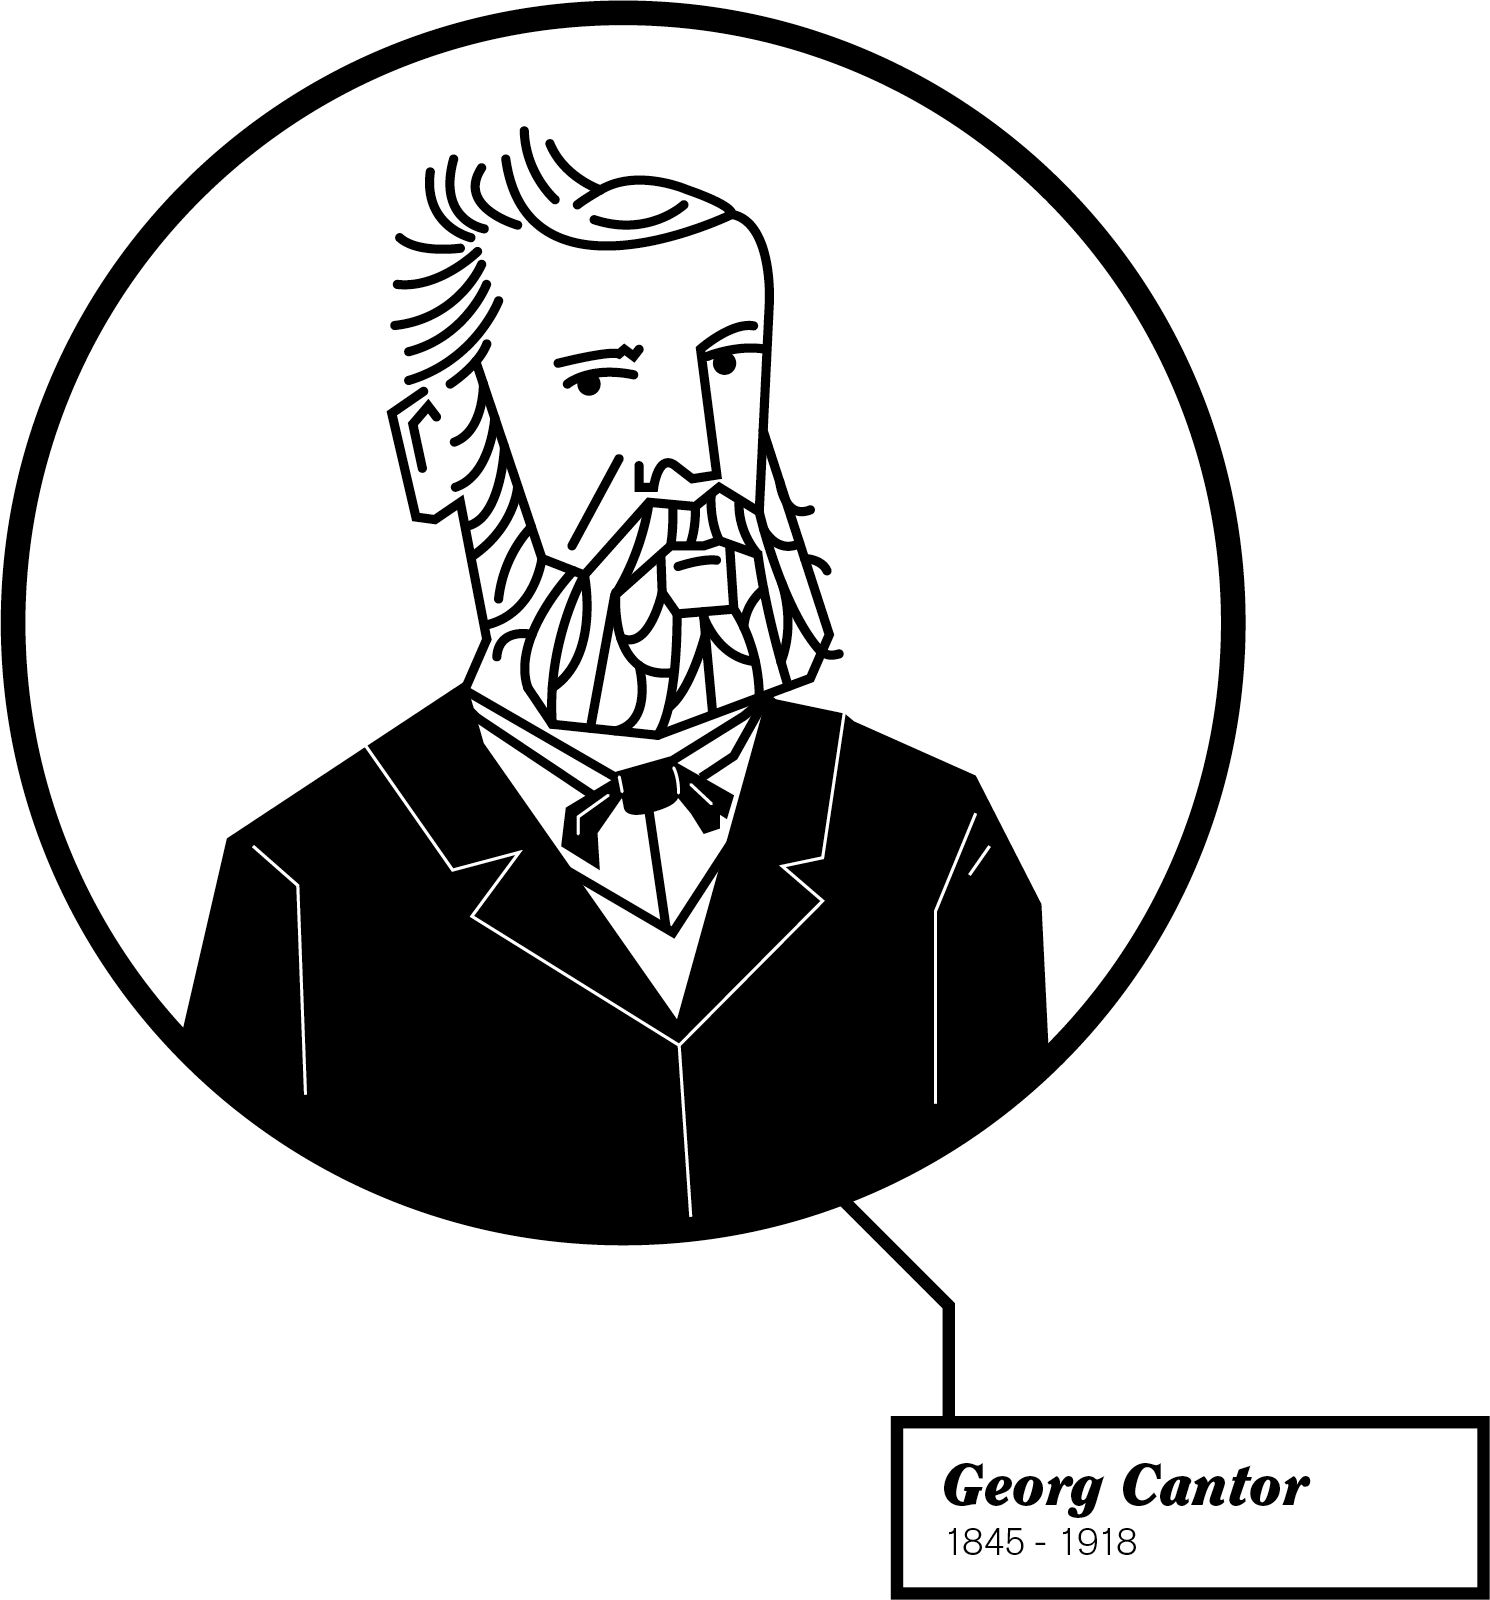
\includegraphics[width=\textwidth]{illustrations/CantorChapter}
\vfill
\mainmatter
\olimport*[sets-functions-relations]{sets-functions-relations}

\cleartoverso
\ifodd\value{page}\stepcounter{page}\fi
\thispagestyle{empty}
\ \vfill
\noindent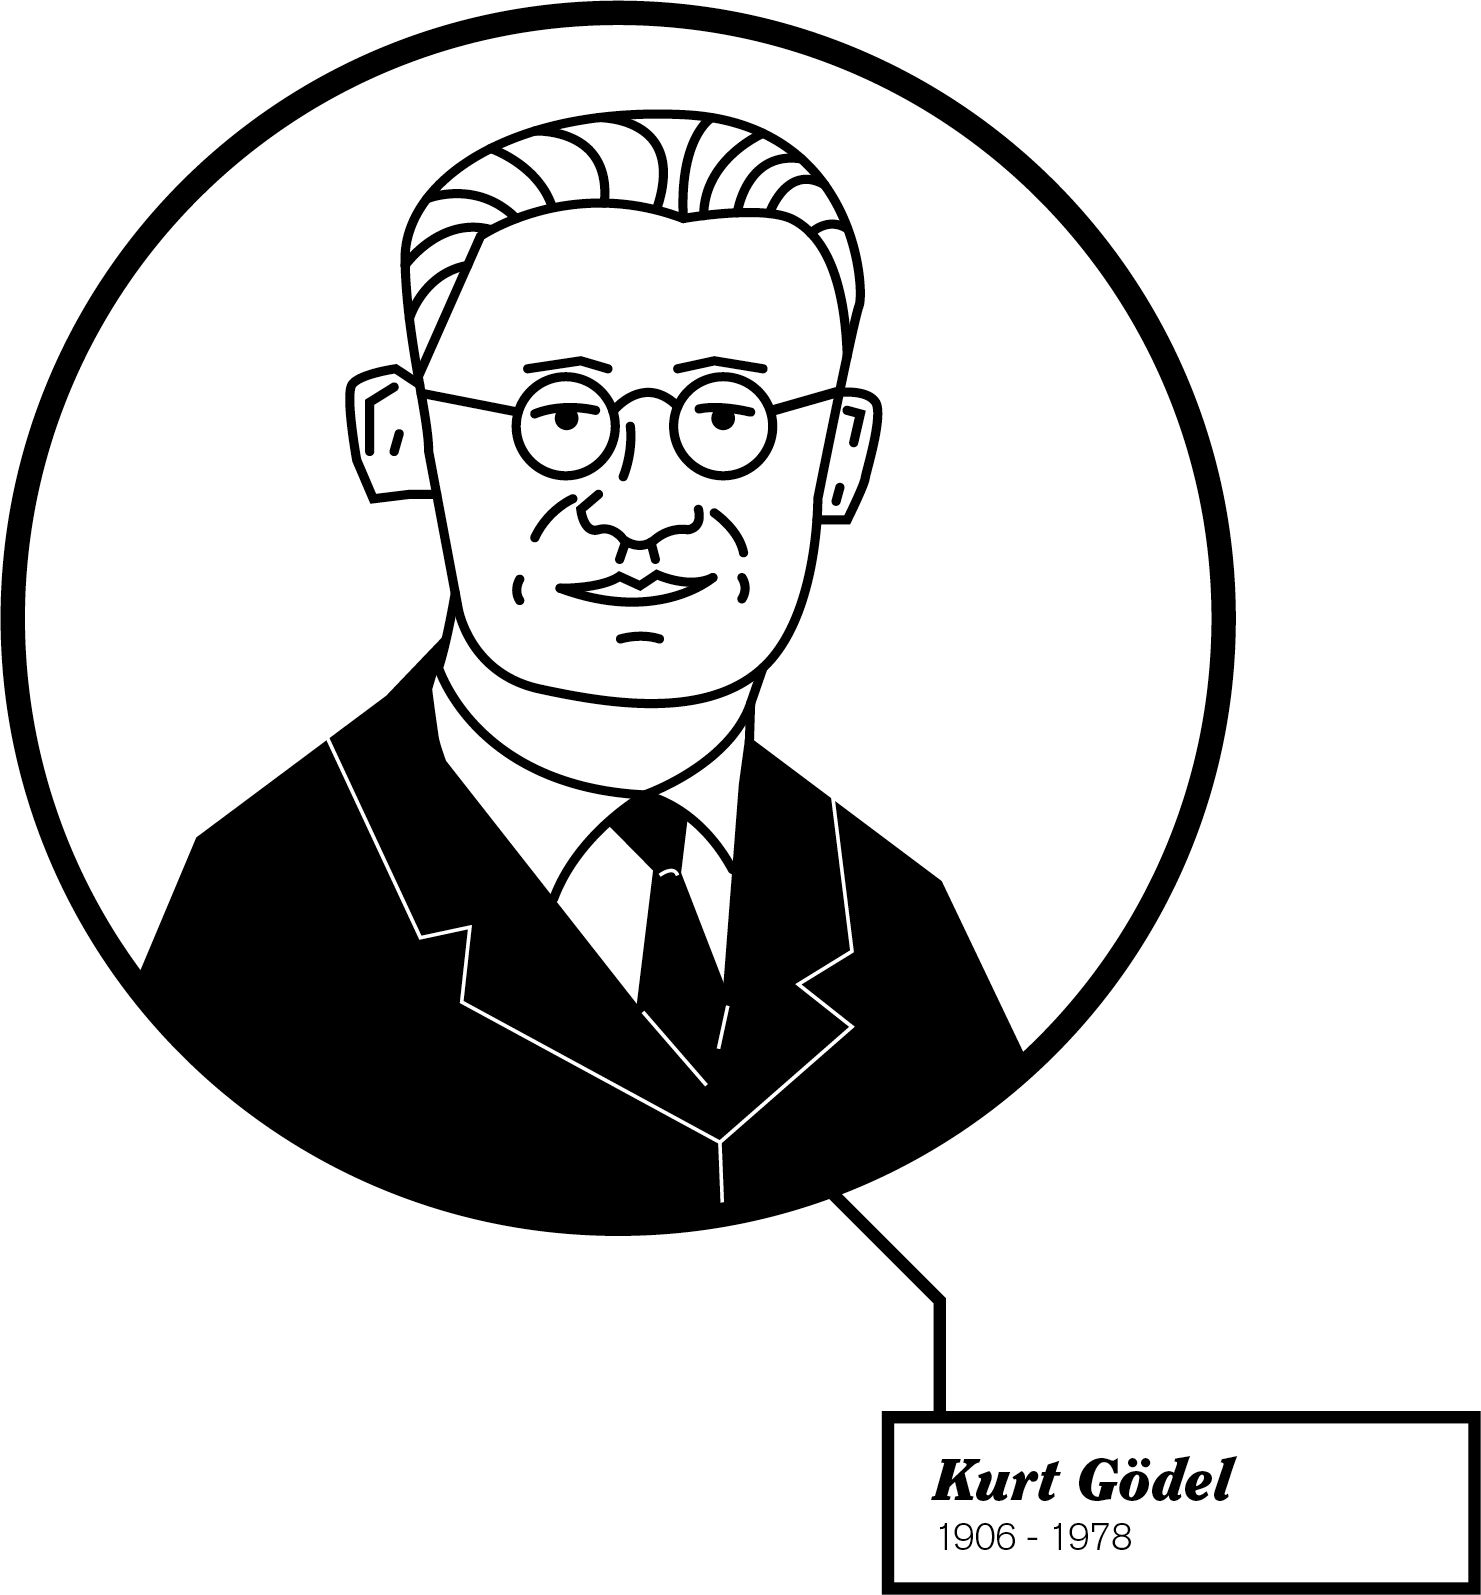
\includegraphics[width=\textwidth]{illustrations/GodelChapter}
\vfill
\olimport*[first-order-logic]{first-order-logic}

\cleartoverso
\ifodd\value{page}\stepcounter{page}\fi
\thispagestyle{empty}
\ \vfill
\noindent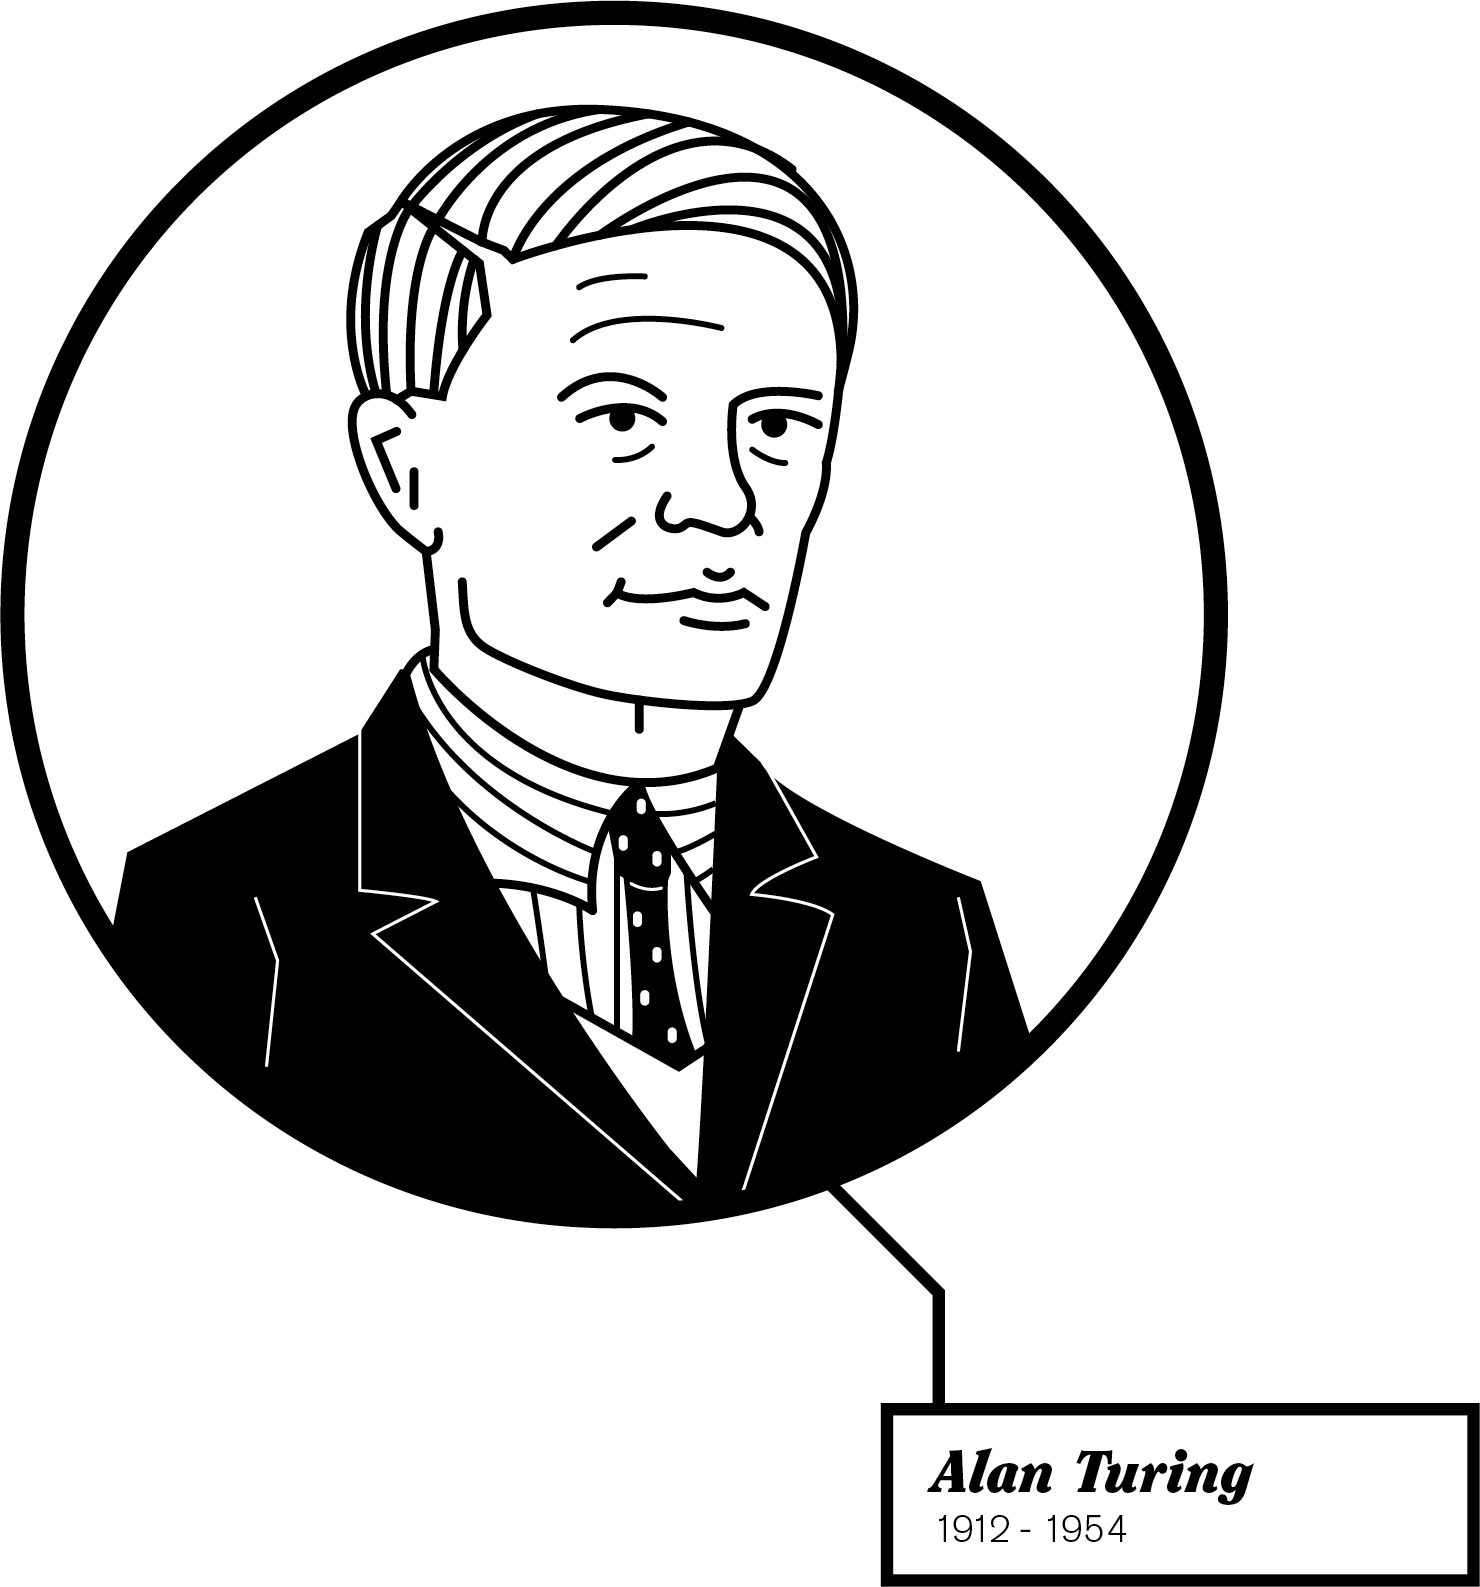
\includegraphics[width=\textwidth]{illustrations/TuringChapter}
\vfill
\olimport*[turing-machines]{turing-machines}

\cleartoverso
\ifodd\value{page}\stepcounter{page}\fi
\thispagestyle{empty}
\ \vfill
\noindent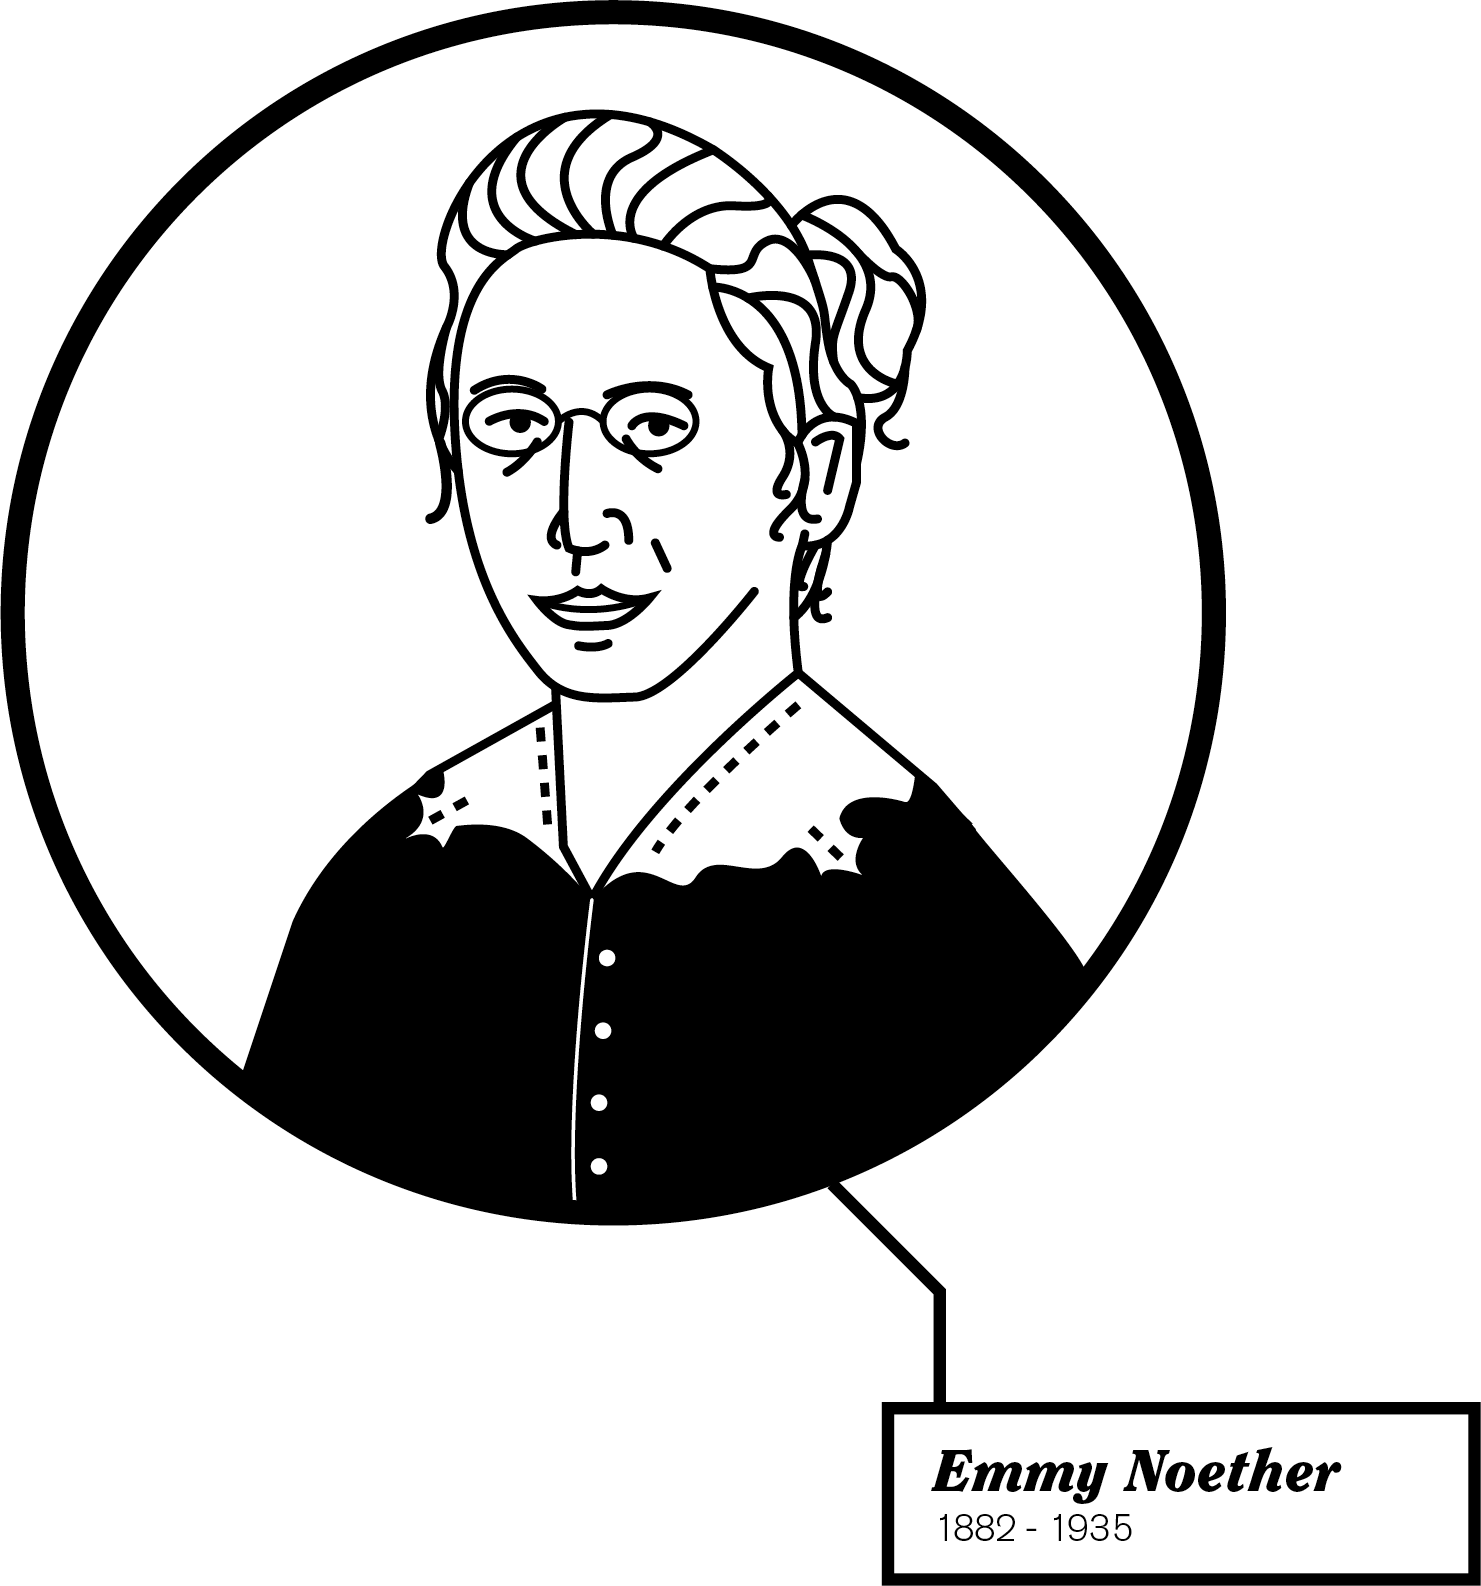
\includegraphics[width=\textwidth]{illustrations/NoetherChapter}
\vfill
\appendix
\olimport*[methods/proofs]{proofs}
\olimport*[methods/induction]{induction}

\stopproblems
\def\ifproblems#1{}
\def\figurename{આકૃતિ}
\setlength{\olphotowidth}{.45\textwidth}
\chapter{તર્કશાસ્ત્રીઓનાં જીવનચરિત્રો}
\olimport*[history/biographies]{georg-cantor}
\olimport*[history/biographies]{alonzo-church}
\olimport*[history/biographies]{gerhard-gentzen}
\olimport*[history/biographies]{kurt-goedel}
\olimport*[history/biographies]{emmy-noether}
\olimport*[history/biographies]{bertrand-russell}
\olimport*[history/biographies]{alfred-tarski}
\olimport*[history/biographies]{alan-turing}
\olimport*[history/biographies]{ernst-zermelo}
\olimport*[reference/greek-alphabet]{greek-alphabet}

\glsaddall
\printglossary[title=પરિભાષાકોશ,toctitle=પરિભાષાકોશ]
\clearpage
\photocredits
\bibliographystyle{natbib-oup}
\bibliography{\olpath/bib/open-logic}
\olimport*{\olpath/locale/\ollangid/content/open-logic-about}

\end{document}
